\documentclass[10pt]{article}
\usepackage{color}
\usepackage{graphicx} % Required for inserting 
%%\usepackage{algpseudocode} % Include the package for algorithmic environment
\usepackage{algorithm}
\usepackage{booktabs} % For better-quality horizontal lines
\usepackage{algpseudocode}
\usepackage{multirow}
\usepackage{threeparttable} % For table notes
\usepackage{array} % For table formatting

\usepackage{setspace}
\usepackage{float} % add this in your preamble
\usepackage{amsmath}
\usepackage{tabularx}

\usepackage[round]{natbib}

\usepackage{multirow}
\usepackage{fourier} 
\usepackage{booktabs}
\usepackage{array}
\usepackage{makecell}
\usepackage[font={small,it}]{caption}
\usepackage[utf8]{inputenc}
\usepackage{mathtools}
\usepackage{subcaption}
\usepackage{tabstackengine}
\usepackage[toc,page]{appendix}
\usepackage{graphicx, fullpage, verbatim, amsmath}
\usepackage{url, amsfonts, amssymb, amsthm,color, enumerate}
\usepackage{placeins, listings, textcomp, mathtools, multicol, tikz}
\usepackage{ dsfont }
\usepackage{bm}
\newcommand\fixed{^\dagger}


\TABstackMath

\doublespacing
% Language setting
% Replace `english' with e.g. `spanish' to change the document language
\usepackage[english]{babel}

% Set page size and margins
% Replace `letterpaper' with `a4paper' for UK/EU standard size
\usepackage[a4paper,top=2cm,bottom=2cm,left=3cm,right=3cm,marginparwidth=1.75cm]{geometry}

% Useful packages
\usepackage{graphicx}
\bibliographystyle{apalike}
\usepackage[colorlinks=true,citecolor=blue]{hyperref}
\newcommand\choleraDeath{\delta_{C}}

% Using \doublespacing in the preamble 
% changes the text to double-line spacing
\doublespacing


\title{%
  \textbf{\LARGE{PAL versus SMC: Two Approaches in Compartmental Modeling}} \\
  \large A case study with rotavirus in Germany during 2001-2008 \\}
\author{\large Yize Hao\\[0.5cm]{\median Supervisor: Prof. Edward Ionides \\ 
Graduate Student Mentor: Aaron Abkemeier}
    }
    \date{Submitted: April 23, 2024 \\ This version: May 31, 2024}

\begin{document}

\maketitle

\begin{abstract}
Partially Observed Markov Process (POMP) models have been extensively employed in epidemiological modeling over the past several decades to understand disease patterns and inform policy-making. Although the observation density is typically assumed to be known or at least can be evaluated point-wisely, the latent Markovian models lack closed-form expressions for initial density and transition kernels, making it challenging to compute the likelihood for POMP models with complex latent models. Recently, a novel approach (Poisson Approximate Likelihood, PAL) was introduced by \cite{wwr}, which employs a Poisson approximation to posterior densities, offering a fast and consistent approximation for the likelihood function. \cite{wwr} claimed that their method, along with its associated model, improved the maximum likelihood estimation compared to traditional sequential Monte Carlo (SMC) methods used in \cite{stocks} when applied to the German rotavirus, by approximately 3200 log-likelihood units. However, our analysis of comparing two methods applied to the model for the same rotavirus dataset reveals that the improvement of 3200 log-likelihood units results from the use of two different datasets differed by a scaling factor. Moreover, although PAL and SMC are two ways of approximating the likelihood, within the framework of models compatible with PAL, when computation time is preferred, PAL is recommended but it may suffer from a likelihood shortfall, which can't be overcome in general. When the model is misspecified for certain time points, SMC may fail, and PAL is possible to approximate the likelihood. When computational time is not a critical factor and the model is correctly specified, sequential Monte Carlo methods are recommended. 
\end{abstract}

\noindent\textbf{Keywords:} epidemiology; compartmental model; state-space model; sequential Monte Carlo; likelihood-based inference

\section{Introduction}

Understanding dynamic diseases is critical for public health and policy-making. Traditional time series models, such as the TSIR model \citep{TSIR1, TSIR_package}, are valuable for predicting and forecasting the transmission scale of specific infectious diseases, as well as for estimating critical parameters such as the basic reproduction number $R_0$ and the force of infection. However, these models still fail to provide a sufficiently clear and straightforward understanding of the disease's transmission dynamics. Therefore, modeling the epidemiology data differently is necessary. Here, we seek an alternative approach --- Partially Observed Markov Process (POMP) models with compartmental modeling in the latent process, which is one of the most widespread models for understanding the dynamics of infectious diseases and epidemiology data in the recent several decades \citep{mseh, HULIN2000197, daihai, plospomp, stocks, wastewater, daihai2,wwr}. However, when there is a desire for models to more closely resemble reality—namely, moving beyond linear Gaussian assumptions—traditional filtering methods such as the Kalman Filter \citep{kalman1960} and the Ensemble Kalman Filter \citep{ensembkal, ensemkalman2} become unsuitable. This complexity arises because many diseases are inherently more complicated; they are often modeled as nonlinear, non-Gaussian, high-dimensional, and highly stochastic POMP models with several compartments in the latent process. 


POMP models are defined by their initial conditions, transition kernels, and observation densities. Though the observation density is always assumed to be mathematically evaluatable, the latent Markovian models have neither a closed-form initial density nor transition kernels. Therefore, the likelihood often is hard to retrieve when such a model is fairly complicated. However, as proposed by \cite{Kitagawa1987-fr, gordon1993, Kitagawa1996-wa}, Monte Carlo methods can be applied sequentially to approximate the posterior distribution, as well as the likelihood function. This is the so-called and widely-used sequential Monte Carlo method for filtering general models as long as one can simulate from the latent Markovian model, which is based on the idea of Sampling-Importance-Resampling \citep{Rubin1987}. 

Owing to the unique characteristics of POMP models, which we will introduce subsequently, these models have gained significant importance and have been extensively applied in engineering and related disciplines, such as speech word identification \citep{rabiner1989}, target positioning and velocity estimation in radar systems \citep{gordon1993, avitzour1995}, volatility estimation in economic time series \citep{Pitt1999-volatility}, and structural type prediction in protein secondary structures \citep{Schmidler2000-protein}. In these models, the unobserved signal process $\{x_n: n \in \mathds{N}\}, x_n \in \mathcal{X}$, represents the true underlying signal, where $\mathcal{X}$ denotes the space where the state vectors live. A key example is the widely utilized SIR model for infectious disease modeling, which categorizes individuals into three compartments: S (susceptible), I (infectious), and R (recovered) \citep{daihai, seircov, SEIRmodel}. In this case, $\mathcal{X} = \mathds{N}^3$, where $\mathds{N}$ is the set of natural numbers. $x_n =  (S_n, I_n, R_n)$ where $S_n$, $I_n$, and $R_n$ indicate the number of individuals in each compartment at time $n$. However, what is observable is $\{y_n|n\in \mathds{N}\}, y_n \in \mathcal{Y}$, which depends only on $\{x_n: n\in\mathds{N}\}, x_n \in \mathcal{X}$ and always includes noise components. In the above SIR example, $\mathcal{Y} = \mathds{N}$ since $y_n$, our data, is the observed number of cases at time $n$. Therefore, accurately retrieving the values of $\{x_n: n\in\mathds{N}\}, x_n \in \mathcal{X}$ based on the observations $y_{1:N}$ is crucial, a challenge commonly referred to as a filtering problem. This entails filtering out the noise to recover the posterior distribution of $x_{1:n}$ given $y_{1:n}, n\in\mathds{N}$, a problem widely considered in Bayesian statistics. \citep{gordon1993, geweke1989, bayesiandoucet, pmcmc}


When inference and estimation of parameters are of interest, likelihood maximization methods are particularly challenging when the likelihood function is mathematically intractable, as detailed in \cite{Breto2019-sz, iteratedfiltering, daihai}. These methods often rely solely on the "plug-and-play" property, which depends only on simulations from the latent process model. Conversely, when the likelihood function is accessible, either through integration or approximation, methods such as the gradient ascent algorithm \citep{Lemarechal2012, Hadamard1908, Courant1943} and the Stochastic EM algorithm \citep{stochasticEM} can be effectively utilized.

Next, we introduce the POMP model in general and then review two different filtering methods that were proposed and compared in \cite{wwr}. Subsequently, we will discuss the model specifically used for the German rotavirus from 2001 to 2008 as a case study, which will enhance understanding of the two methods and, more importantly, provide guidance on whether and when one should use them.




\section{Methodology}


\begin{center}
\begin{tabular}{|c c|} 
 \hline
 Notation & Description  \\ [0.5ex] 
 \hline
 $\theta, \phi$ & Parameters, usually $\theta, \phi \in \mathds{R}^p, p\geq 1$\\ 
 \hline
 $f(\cdot; \theta),p(\cdot; \theta)$ & \makecell{Probability density functions parametrized by parameter $\theta$ of \\continuous and discrete random variables respectively}  \\
 \hline
 $X_{1:n}$ & State variable from time 1 to n.  \\
 \hline
 $Y_{1:n}$ & Observation variable from time 1 to n. \\
 \hline
 $x_{1:n}$ & The realization of the state variable from time 1 to n.  \\
 \hline
 $y_{1:n}$ & The realization of the observation variable from time 1 to n.  \\
 \hline
 $\mathcal{L}(\theta|\cdot)=f(\cdot|\theta)$ & The likelihood function at parameter $\theta$ given data.  \\
 \hline
 $\ell(\theta|\cdot)=logf(\cdot|\theta)$ & The log-likelihood function at parameter $\theta$ given data.  \\
 \hline
\end{tabular}
\end{center}

\subsection{The Partially Observed Markov Process (POMP) Model}
The Partially Observed Markov Process (POMP) model \citep{daihai}, also known as the state-space model (SSM), or the Hidden Markov Model (HMM), is a time series model consisting of processes \citep{Chopin, liujun, Doucet}: A latent process/ state model, written as $x_n \sim f_{X_n|X_{n-1}}(\cdot|x_{n-1},\theta)$ and an observation/ measurement model, written as $y_n \sim f_{Y_n|X_n}(\cdot|x_n,\theta)$. Here, we only consider the discrete-time representation. Where $\{x_n: n\in\mathds{N}\}, x_n \in \mathcal{X}$ denotes the hidden or latent states representing the unobserved signal. These states are treated as missing data within our model and are of interest, a point that will be elaborated upon subsequently. And $\{y_n|n\in \mathds{N}\}, y_n \in \mathcal{Y}$ are called observations and are our actual observed data. The latent process is modeled as a Markov process, i.e. $\{x_n: n\in\mathds{N}\}$ has the Markovian property: $f_{X_n|X_{1:n-1}}(x_n|x_{1:n-1}, \theta)=f_{X_n|X_{n-1}}(x_n|x_{n-1},\theta)$ with initial distribution $f_{X_0}(x_0;\theta)$ and the transition kernel $f_{X_n|X_{n-1}}(x_n|x_{n-1},\theta)$. $\{y_n|n\in \mathds{N}\}$ are conditionally independent given the state variables $\{x_n: n\in\mathds{N}\}$, and if $\{x_n: n\in\mathds{N}\}$ were given, $y_n$ only depends on $x_n$ in the way that $y_n \sim f_{Y_n|X_{n}}(y_n|x_n,\theta)$. And $f_{Y_n|X_{n}}(y_n|x_n,\theta)$ is called the observation/ measurement density. Such conditions are visualized by Figure \ref{fig1}.


Consequently, the likelihood function can be written as:
\vspace{-2mm}
\begin{align} 
\mathcal{L}(\theta|y_{1:N}) &= f_{Y_{1:N}}(y_{1:N}; \theta) \\
&= \int f_{Y_{1:N},X_{0:N}}(y_{1:N}, x_{0:N};\theta) dx_{0:N} \\
&= \int f_{X_0}(x_0;\theta) \prod_{n=1}^N
f_{Y_n|X_n}(y_n|x_n,\theta)
f_{X_n|X_{n-1}}(x_n|x_{n-1},\theta) dx_{0:N} 
\end{align}

\begin{figure}[h]
\centering
\includegraphics[width=0.8\textwidth]{pic2.png}
\caption{\label{fig:hiddenmarkovmodel}Partially Observed Markov Process (POMP) Model \citep{gettingstartpomp}}
\label{fig1}
\end{figure}

However, $f_{X_0}(x_0;\theta)$, and $f_{X_n|X_{n-1}}(x_n|x_{n-1};\theta)$ doesn't always have a closed-form expression, especially for compartmental modeling for complex epidemiology data. Therefore, evaluating the likelihood by simply calculating the integral directly is nearly impossible. Here, for estimation and inference, we review two methods for calculating the likelihood.


\subsection{Sequential Monte Carlo/ Particle Filtering (SMC)}

The sequential Monte Carlo (SMC), also known as Particle Filtering, has been widely used with various variants developed over recent decades for posterior density approximation, including $f_{X_n|Y_{1:n-1}}(x_n|y_{1:n-1}, \theta)$ and $f_{X_n|Y_{1:n}}(x_n|y_{1:n},\theta)$, as well as for likelihood approximation. Theoretical foundations are discussed in \cite{Chopin, Doucet, liujun}, and R packages implementing SMC are detailed in \cite{pomppackagepaper}. Here, we introduce the basic concept of how SMC functions for likelihood approximation to serve our specific objectives.

Suppose we are interested in computing the likelihood for such POMP models. Recall that:
\begin{align*} 
\mathcal{L}(\theta|y_{1:N}) &= f_{Y_{1:N}}(y_{1:N}; \theta) \\
&=  \prod_{n=1}^N f_{Y_n|Y_{1:n-1}}(y_n|y_{1:n-1}, \theta) \\
&=  \prod_{n=1}^N \mathcal{L}_n(\theta) \\
\end{align*}
\vspace{-20mm}

where we let $f_{Y_n|Y_{1:n-1}}(y_n|y_{1:n-1}, \theta) = f_{Y_1}(y_1| \theta)$, when $n=1$, and $\mathcal{L}_n(\theta) := f_{Y_n|Y_{1:n-1}}(y_n|y_{1:n-1}, \theta)$.
Thus, we merely need to compute $\mathcal{L}_n(\theta)$. By the following formula:
\begin{align*}
    \mathcal{L}_n(\theta) &= f_{Y_n|Y_{1:n-1}}(y_n|y_{1:n-1}, \theta) \\
    &=  \int f_{Y_n,X_n|Y_{1:n-1}}(y_n, x_n|y_{1:n-1}, \theta)dx_n \\
    &=  \int f_{Y_n|X_{n},Y_{1:n-1}}(y_n| x_n,y_{1:n-1}, \theta)f_{X_n|Y_{1:n-1}}(x_n|y_{1:n-1}, \theta)dx_n \\
    & = \int f_{Y_n|X_{n}}(y_n|x_n, \theta)f_{X_n|Y_{1:n-1}}(x_n|y_{1:n-1}, \theta)dx_n \\
    &= \mathds{E}_{X_n|Y_{1:n-1}}[f_{Y_n|X_{n}}(y_n|X_n,\theta)|y_{1:n-1},\theta]
\end{align*}

by the conditional independency of $y_n$ given $x_n$. Then if we can sample $x^{(i)}_n \sim p(x_n|y_{1:n-1}, \theta)$, by Law of Large Numbers, we have 
\vspace{-1mm}
\begin{align*}
\frac{1}{J}\sum_{i=1}^{J}f_{Y_n|X_{n}}(y_n|x^{(i)}_n,\theta) \xrightarrow{\: J \to \infty \: } &\int f_{Y_n|X_{n}}(y_n|x_n, \theta)f_{X_n|Y_{1:n-1}}(x_n|y_{1:n-1}, \theta)dx_n \\
= &f_{Y_n|Y_{1:n-1}}(y_n|y_{1:n-1}, \theta) 
\end{align*}
 
Therefore, our objective shifts to sequentially sampling $x_n^{(i)}$ from $f_{X_n|Y_{1:n-1}}(x_n|y_{1:n-1}, \theta)$ for each $n \geq 1$. Sampling sequentially means that we don't want to sample a whole different set of $\{x_{n+1}^{(i)}\}_i$ whenever a new observation $y_{n+1}$ is available. This can be achieved by the sequential Monte Carlo technique as shown in Algorithm \ref{alg1}.

\vspace{3mm}


\begin{algorithm}
\caption{Sequential Monte Carlo (SMC, or particle filter)}
\label{alg1}
\begin{algorithmic}[1]
\Statex \textbf{Input: }Simulator for $f_{X_n|X_{n-1}}(x_n | x_{n-1}; \theta)$; evaluator for $f_{Y_n|X_n}(y_n | x_n; \theta)$; simulator for $f_{X_0}(x_0;\theta)$; parameter, $\theta$; data, $y_{1:N}$; number of particles, $J$.
\For{$n$ in $1:N$}
    \State Simulate for prediction: $X_{n,j}^P \sim f_{X_n|X_{n-1}}(\cdot | X_{n-1,j}^F;\theta)$ for $j$ in $1:J$.
    \State Evaluate weights: $w(n,j) = f_{Y_n|X_n}(y_n^*|X_{n,j}^P;\theta)$ for $j$ in $1:J$.
    \State Normalize weights: $\tilde{w}(n,j) = \frac{w(n,j)}{\sum_{m=1}^J w(n,m)}$.
    \State Apply select indices $k_{1:J}$ with $P[k_j = m] = \tilde{w}(n,m)$.
    \State Resample with replacement: set $X_{n,j}^F = X_{n,k_j}^P$ for $j$ in $1:J$.
    \State Compute conditional log likelihood: $\hat{l}_{n|1:n-1} = \log \left( J^{-1} \sum_{m=1}^J w(n,m) \right)$.
\EndFor
\end{algorithmic}
\textbf{output:} Log likelihood estimate, $\hat{l}(\theta) = \sum_{n=1}^N \hat{l}_{n|1:n-1}$; filter sample, $X_{n,1:J}^F$, for $n$ in $1:N$. \\
\textbf{complexity:} $O(J)$
\end{algorithm}

Moreover, one can show that $X_{n,j}^P, j=1,2...,J$ is an approximation of the prediction distribution $f_{X_{n}|Y_{1:n-1}}(x_{n}|y_{1:n-1})$. After reweighting, $X_{n,j}^F, j=1,2...,J$ is an approximation of the filtering distribution $f_{X_{n}|Y_{1:n}}(x_{n}|y_{1:n})$, see \cite{gordon1993, Smith1992-st}. 

\vspace{3mm}
Another way of computing the likelihood is by noticing: 
\vspace{-3mm}
\begin{align}\label{eq4-6}
&\textit{Prediction Formula: }     &&f_{X_n|Y_{1:n-1}}(x_n|y_{1:n-1})=\int f_{X_n|X_{n-1}}(x_n|x_{n-1})f_{X_{n-1}|Y_{1:n-1}}(x_{n-1}|y_{1:n-1})dx_{n-1}\\
&\textit{Filtering Formula: } &&f_{X_n|Y_{1:n}}(x_n|y_{1:n})=\frac{f_{Y_n|X_n}(y_n|x_n)f_{X_n|Y_{1:n-1}}(x_n|y_{1:n-1})}{f_{Y_n|Y_{1:n-1}}(y_n|y_{1:n-1})} \\
&\textit{Conditional Likelihood: } &&f_{Y_n|Y_{1:n-1}}(y_n|y_{1:n-1}) =\int f_{Y_n|X_n}(y_n|x_n)f_{X_n|Y_{1:n-1}}(x_n|y_{1:n-1})d{x_n}
\end{align}




When $f_{X_n|Y_{1:n}}(x_n \mid y_{1:n})$ and $f_{X_n|Y_{1:n-1}}(x_n \mid y_{1:n-1})$ are known functions of $n$, the likelihood can also be computed for all $n$, as these probabilities are inherently related to each other. 

Since
\vspace{-3mm}
\begin{align*}
    f_{X_{n-1}|Y_{1:n-1}}(x_{n-1}|y_{1:n-1}) \xrightarrow{\text{prediction}} f_{X_n|Y_{1:n-1}}(x_n|y_{1:n-1}) \xrightarrow{\text{update}} f_{X_n|Y_{1:n}}(x_{n}|y_{1:n}) 
\end{align*}



However, the evaluation of those integrals is almost impossible due to their complex and high-dimensional nature. Thus obtaining approximations for this distribution is more welcome \citep{Doucet}. 

\subsection{Poisson Approximate Likelihood (PAL)}

Denote $p_{X_n|Y_{1:n-1}}(x_n|y_{1:n-1})$ as the prediction density; $p_{X_n|Y_{1:n}}(x_n|y_{1:n})$ as the filtering density. Suppose $\{X_n: n\in \mathds{N}\}$ and $\{Y_n: n\in \mathds{N}\}$ are discrete random variables, with $\mathcal{X}=\mathds{N}^m$,$\mathcal{Y}=\mathds{N}$, and $m \in \mathds{N}$ is the number of compartments, by very minimum algebra, we have:
\vspace{-3mm}
\begin{align*}
&\textit{Prediction Formula: }     &&p_{X_n|Y_{1:n-1}}(x_n|y_{1:n-1})=\sum_{x_{n-1}\in \mathds{N}_0^m}p_{X_n|X_{n-1}}(x_n|x_{n-1})p_{X_{n-1}|Y_{1:n-1}}(x_{n-1}|y_{1:n-1}) \\
&\textit{Filtering Formula: } &&p_{X_n|Y_{1:n}}(x_n|y_{1:n})=\frac{p_{Y_n|X_n}(y_n|x_n)p_{X_n|Y_{1:n-1}}(x_n|y_{1:n-1})}{p_{Y_n|Y_{1:n-1}}(y_n|y_{1:n-1})} \\
&\textit{Conditional Likelihood: } &&p_{Y_n|Y_{1:n-1}}(y_n|y_{1:n-1}) =\sum_{x_n\in \mathds{N}_0^m}f_{Y_n|X_n}(y_n|x_n)p_{X_n|Y_{1:n-1}}(x_n|y_{1:n-1})
\end{align*}
which is a discrete representation of Eq. (\ref{eq4-6})-(6).

\vspace{4mm}
Given $p_{X_0}(x_0), p_{X_n|X_{n-1}}(x_n|x_{n-1})$, and $p_{Y_n|X_{n}}(y_n|x_{n})$ for $n\geq1$, we can approximate $p_{X_n|Y_{1:n-1}}(x_n|y_{1:n-1})$, $p_{X_n|Y_{1:n}}(x_n|y_{1:n})$, and $p_{Y_n|Y_{1:n-1}}(y_n|y_{1:n-1})$ at any time $n\geq1$ and then use the above quantities to update $p_{X_n|X_{n-1}}(x_n|x_{n-1}), p_{X_n|Y_{1:n}}(x_n|y_{1:n})$, and $p_{X_n|Y_{1:n}}(x_n|y_{1:n})$ at the next given time $n+1$. The Poisson Approximate Likelihood (PAL) method assumes and approximates them by a vector Poisson approximation. 

\newpage
\begin{enumerate}
    \item 
In the latent process model: 
\vspace{-2mm}
\begin{enumerate}
    \item $\bm{\delta_t}$ be the death rate vector;
    \item $\bm{\alpha_t}$ be the birth rate vector of m compartments;
    \item $\bm{K_{t, \eta}}$ be the row stochastic matrices;
\end{enumerate}
\vspace{-2mm}
Then the one-step transition of the latent process can be described as:

$\bm{x_t} = \bm{\tilde{x}_t} + \bm{\hat{x}_t}$, where $\bm{\tilde{x}}$ is obtained by $\bm{\bar{x}_{t-1}} \sim Binom(\bm{x}_{t-1}, \bm{1- \delta_t})$ and $\bm{\tilde{x}_t}$ is equal to the one-step transition of $\bm{\bar{x}_{t-1}}$ according to the transition kernel $\bm{K_{t-1, \eta}}$. And $\bm{\hat{x}_t} \sim Pois(\bm{\alpha}_t)$ is the importing birth, which is considered as stochastic noise. 
\vspace{-3mm}
\item In the observation model:
\vspace{-2mm}
    \begin{enumerate}
        \item $\bm{q_t}\in [0,1]^m$ be the observing probability, where $m$ is the number of compartments;
        \item $\bm{G_t}$ be the misreporting kernel, where non-zero off-diagonal entries indicate misreporting. 
        \item $\bm{\kappa_t}$ be the observation error rate.
    \end{enumerate}
\vspace{-2mm}
    Then $\bm{y_t} = \bm{\tilde{y}}_t + \bm{\hat{y}}_t$, where $\bm{\hat{y}}_t \sim Binom(\bm{x_t}, \bm{q_t})$. And $\bm{\hat{y}}_t \sim Pois(\bm{\kappa_t})$ is the observation error.
    
\end{enumerate}

A novel method suggested by \cite{wwr} is that the conditional likelihood of the above compartmental model can be approximated by Poisson densities by the following:


If we assume $p_{X_0}(\bm{x}_0) \approx \operatorname{Pois}(\bm{\lambda}_0)$, where $\bm{\lambda}_0$ is a parameter that characterizes the initial distribution of the numbers of individuals in each compartment. 

Then for $t \geq 1$:

\begin{enumerate}
    \item $p(\bm{x}_t|\bm{y}_{1:t-1}) \approx \operatorname{Pois}(\bm{\lambda}_t)$, where $\bm{\lambda}_t$ :=$(\bm{\bar{\lambda}}_{t-1} \odot \bm{\delta_t})^\intercal \bm{K_{t,\eta(\bm{\bar{\lambda}}_{t-1} \odot \bm{\delta_t})}} + \bm{\alpha}_t$     
    \item 

    $p\left(\mathbf{x}_t \mid \mathbf{y}_{1: t}\right) \approx \operatorname{Pois}\left(\bm{\bar{\lambda}}_t\right), \quad \bm{\bar{\lambda}}_t:=\left[\mathbf{1}_m-\mathbf{q}_t+\left(\left\{\mathbf{y}_t^{\top} \oslash\left[\left(\mathbf{q}_t \odot \bm{\lambda}_t\right)^{\top} \mathbf{G}_t+\boldsymbol{\kappa}_t^{\top}\right]\right\}\left[\left(\mathbf{1}_m \otimes \mathbf{q}_t\right) \odot \mathbf{G}_t^{\top}\right]\right)^{\top}\right] \odot \bm{\lambda}_t$

    \item $p(\mathbf{y}_t|\bm{y}_{1:t-1}) \approx \operatorname{Pois}\left(\bm{\mu}_t\right)$, where $\bm{\mu}_t = \left[(\bm{\lambda}_t \odot \mathbf{q}_t)^{\top} \mathbf{G}_t\right]^{\top}+\boldsymbol{\kappa}_t$.
\end{enumerate}

Therefore, the algorithm of the approximated likelihood is:
\vspace{2mm}
\begin{algorithm}
\caption{Poisson Approximate Likelihood (PAL)}
\begin{algorithmic}[1]
\Statex \textbf{Initialize: }$\bar{\lambda}_0 \leftarrow \lambda_0$.
\For{$t$ in $1:N$}
    \item \quad $\lambda_t \leftarrow\left[\left(\bar{\lambda}_{t-1} \odot \delta_t\right)^{\top} \mathbf{K}_{t, \boldsymbol{\eta}\left(\bar{\lambda}_{t-1} \odot \delta_t\right)}\right]^{\top}+\boldsymbol{\alpha}_t$
    \item \quad $\bar{\lambda}_t \leftarrow\left[\mathbf{1}_m-\mathbf{q}_t+\left(\left\{\mathbf{y}_t^{\top} \oslash\left[\left(\mathbf{q}_t \odot \lambda_t\right)^{\top} \mathbf{G}_t+\boldsymbol{\kappa}_t^{\top}\right]\right\}\left[\left(\mathbf{1}_m \otimes \mathbf{q}_t\right) \odot \mathbf{G}_t^{\top}\right]\right)^{\top}\right] \odot \lambda_t$
    \item \quad $\boldsymbol{\mu}_t \leftarrow\left[\left(\lambda_t \odot \mathrm{q}_t\right)^{\top} \mathbf{G}_t\right]^{\top}+\boldsymbol{\kappa}_t$
    \item \quad $\ell\left(\mathbf{y}_t \mid \mathbf{y}_{1: t-1}\right) \leftarrow-\boldsymbol{\mu}_t^{\top} \mathbf{1}_m+\mathbf{y}_t^{\top} \log \left(\boldsymbol{\mu}_t\right)-\mathbf{1}_m^{\top} \log \left(\mathbf{y}_{t} !\right)$
\EndFor
\end{algorithmic}
\end{algorithm}

\newpage 

To account for overdispersion within the model, \cite{wwr}'s approach entails the introduction of a prior distribution over the parameters. If we separate parameters into two parts i.e. $\theta=[\vartheta, \bar{\theta}_{1:t}]$ where $\vartheta$ are either fixed or to be estimated and $\bar{\theta}_{1:t}$ are to be integrated out and $\bar{\theta}_{1:t} \sim f(\cdot|\phi)$, the prior distribution for $\bar{\theta}_{1:t}$, where $\phi$ are hyperparameters. These parameters $\bar{\theta}_{1:t}$ are then integrated out by importance sampling techniques with proposal distribution $\pi(\cdot|\cdot)$, yielding a marginal distribution of the data that reflects the overdispersion. The procedure is delineated in the following algorithm:

\vspace{3mm}

\begin{algorithm}[H]
\caption{PALSMC}
\begin{algorithmic}[1]
\Statex \textbf{Input: } Proposal distribution $\pi(\cdot|\cdot)$, number of particles J, parameter $[\vartheta, \phi]$
\Statex \textbf{Initialize: }$\bar{\lambda}^{(i)}_0 \leftarrow \lambda_0$, for $i =1,2,...,J$.
\For{$t$ in $1:N$}
    \For{$i= 1,2,...,J$}
    \State $\bar{\theta}^{(i)}_{1:t} \sim \pi(\cdot|\bar{\theta}^{(i)}_{1:t-1}, \bar{\lambda^{(i)}_{t-1}},y_{1:t})$.
    \State $\boldsymbol{\alpha}_t \leftarrow \boldsymbol{\alpha}_t(\vartheta,\bar{\theta}^{(i)}_{t})$, 
    $\mathbf{K}_{t, \boldsymbol{\eta}} \leftarrow \mathbf{K}_{t, \boldsymbol{\eta}}(\vartheta,\bar{\theta}^{(i)}_{t})$, 
    $\boldsymbol{\delta}_t \leftarrow \boldsymbol{\delta}_t(\vartheta,\bar{\theta}^{(i)}_{t})$, 
    $\boldsymbol{q}_t \leftarrow \boldsymbol{q}_t(\vartheta,\bar{\theta}^{(i)}_{t})$,
    \Statex
    \quad \quad \quad $\boldsymbol{\kappa}_t \leftarrow \boldsymbol{\kappa}_t(\vartheta,\bar{\theta}^{(i)}_{t})$,
    $\boldsymbol{G}_t \leftarrow \boldsymbol{G}_t(\vartheta,\bar{\theta}^{(i)}_{t})$
    \State $\lambda_t \leftarrow\left[\left(\bar{\lambda}_{t-1} \odot \delta_t\right)^{\top} \mathbf{K}_{t, \boldsymbol{\eta}\left(\bar{\lambda}_{t-1} \odot \delta_t\right)}\right]^{\top}+\boldsymbol{\alpha}_t$
    \State $\bar{\lambda}_t \leftarrow\left[\mathbf{1}_m-\mathbf{q}_t+\left(\left\{\mathbf{y}_t^{\top} \oslash\left[\left(\mathbf{q}_t \odot \lambda_t\right)^{\top} \mathbf{G}_t+\boldsymbol{\kappa}_t^{\top}\right]\right\}\left[\left(\mathbf{1}_m \otimes \mathbf{q}_t\right) \odot \mathbf{G}_t^{\top}\right]\right)^{\top}\right] \odot \lambda_t$
    \State $\boldsymbol{\mu}_t \leftarrow\left[\left(\lambda_t \odot \mathrm{q}_t\right)^{\top} \mathbf{G}_t\right]^{\top}+\boldsymbol{\kappa}_t$
    \State $\ell\left(\mathbf{y}_t \mid \mathbf{y}_{1: t-1}, \vartheta, \bar{\theta}^{(i)}_{1:t}\right) \leftarrow-\boldsymbol{\mu}_t^{\top} \mathbf{1}_m+\mathbf{y}_t^{\top} \log \left(\boldsymbol{\mu}_t\right)-\mathbf{1}_m^{\top} \log \left(\mathbf{y}_{t} !\right)$
    \State $\log{w^{(i)}_t} \leftarrow \ell\left(\mathbf{y}_t \mid \mathbf{y}_{1: t-1}, \vartheta, \bar{\theta}^{(i)}_{1:t}\right) + \log{f(\bar{\theta}^{(i)}_{t}|\bar{\theta}^{(i)}_{1:t-1}, \phi)}-\log{\pi(\bar{\theta}^{(i)}_{t}|\bar{\theta}^{(i)}_{1:t-1},\bar{\lambda}^{(i)}_t)}$
    \EndFor
    \State $\hat{\ell}\left(\mathbf{y}_t \mid \mathbf{y}_{1: t-1}, \vartheta, \phi\right) \leftarrow \log\left({\frac{1}{J}\sum_{i=1}^{J}w_{t}^{(i)}}\right)$
    \State $\bar{w}_{t}^{(i)}\leftarrow \frac{w_{t}^{(i)}}{\sum_{j=1}^{J}w_{t}^{(j)}}$
    \State Resample $\{\bar{\theta}^{(i)}_{1:t}, \bar{\lambda}_{t}^{(i)}\}$ according to weights $\{\bar{w}_{t}^{(i)}\}_{i=1}^{J}$
\EndFor
\end{algorithmic}
\end{algorithm}




\section{Model: A Case Study with Rotavirus in Germany: 2001-2008}


\begin{table}[ht]
\centering
\caption{Comparison of Model \& Method Performance \citep{wwr}}
\label{tab:model_performance}
% Increase row height
\renewcommand{\arraystretch}{1.5}
\begin{tabular}{@{}lcc@{}}
\toprule
\textbf{Model} & \textbf{AIC} & \textbf{Ave. comp. time} \\
\midrule
EqEq & 98866.65 & 30 s \\
EqOv & 15154.75 & 2 hr \\
OvOv & 13778.08 & 3 hr \\
\cite{stocks} & 20134.38 & 11 hr \\
\bottomrule
\end{tabular}
\end{table}


Model selection is crucial in epidemiology modeling, as it determines the appropriateness of a model in capturing the complexities of disease transmission dynamics. The Akaike Information Criterion (AIC) represents a mathematical approach used in the selection of models and the evaluation of their structural parsimony. The formula for this criterion is given by.
$$
AIC = 2p - \ell(\hat{\theta})
$$
where $p$ is the number of parameters in the model and $\ell(\hat{\theta})$ is the maximized log-likelihood at the estimates. 

When faced with multiple potential models for a dataset, the optimal choice is the model that yields the lowest AIC value. The AIC not only acknowledges the model's fit, evaluated by the likelihood function but also imposes a penalty that escalates with the number of parameters estimated within the model. This penalization is intended to deter overfitting, which is advantageous because augmenting the parameter count typically enhances the model's fit regardless of its true explanatory power.

Next, we introduce the POMP models used in the analysis, beginning with the latent process model, which follows a Markovian structure and includes nine compartments within $\mathcal{X}$.


\subsection{Latent Process Compartmental Model: The SIRSIRSIR model}

\begin{figure}[h]
\centering
\includegraphics[width=0.85\textwidth]{wwrlatentscheme.png}
\caption{\label{fig:SIRSIRSIR model}SIRSIRSIR model \citep{wwr}}
\end{figure}

Rotavirus disease primarily affects infants and young children, causing gastroenteritis in this age group, and is relatively rare in adults \citep{Lambert2009-it}. Nearly every child contracts rotavirus at least once by the age of five \citep{CDC}. Reinfection can occur since neither natural infection nor vaccination against rotavirus provides complete immunity against future infections \citep{stocks}. Consequently, it is practical to categorize the population into three age groups, leading to a model with nine compartments in total: $S_k$, susceptible; $I_k$, infected; $R_k$, recovered, where $k=1,2,3$ corresponds to the age classes 0-4, 5-59, and 60-99, respectively. The diagram of the latent model is shown in Figure \ref{fig:SIRSIRSIR model}, which is employed by both \cite{wwr} and \cite{stocks}. The model is explained in detail subsequently.

The evolution of the full age-stratified rotavirus latent process model at time $t$ is given by:
\begin{align*}
    S_{1,t+1} &= S_{1,t-1} + A_{1,t} + E_{1,t} - B_{1,t} - F^{(S)}_{1,t}, \\
    I_{1,t+1} &= I_{1,t} + B_{1,t} - C_{1,t} - F^{(I)}_{1,t}, \\
    R_{1,t+1} &= R_{1,t} + C_{1,t} - E_{1,t} - F^{(R)}_{1,t}, \\
    S_{2,t+1} &= S_{2,t} + F^{(S)}_{1,t} + E_{2,t} - B_{2,t} - F^{(S)}_{2,t}, \\
    I_{2,t+1} &= I_{2,t} + F^{(I)}_{1,t} + B_{2,t} - C_{2,t} - F^{(I)}_{2,t}, \\
    R_{2,t+1} &= R_{2,t} + F^{(R)}_{1,t} + C_{2,t} - E_{2,t} - F^{(R)}_{2,t}, \\
    S_{3,t+1} &= S_{3,t} + F^{(S)}_{2,t} + E_{3,t} - B_{3,t} - D^{(S)}_{t}, \\
    I_{3,t+1} &= I_{3,t} + F^{(I)}_{2,t} + B_{3,t} - C_{3,t} - D^{(I)}_{t}, \\
    R_{3,t+1} &= R_{3,t} + F^{(R)}_{2,t} + C_{3,t} - E_{3,t} - D^{(R)}_{t},
\end{align*}

where at time $t$: $A_{1,t} \sim \text{Pois}(\alpha_t)$, for some $\alpha_t \in \mathbb{R}$ represents new births, which is chosen according to historical birth record data; $B_{\cdot,t}$ represents new infectives; $C_{\cdot,t}$ represents recovering individuals; $D_{\cdot,t} \sim \text{Binom}(t-1, 1-\delta)$ represents emigrating (dying) individuals; $E_{\cdot,t}$ represents individuals experiencing waning immunity; and $F_{\cdot,t}$ represents aging individuals.

\[
\left[ \begin{array}{c}
    B_{1,t} \\
    F^{(S)}_{1,t} \\
    S_{1,t} - B_{1,t} - F^{(S)}_{1,t}
\end{array} \right]
\sim \text{Mult} 
\left( \begin{array}{c}
    S_{1,t} 
\end{array}, \left[ \begin{array}{c}
    p_{1,t} \\
    1 - e^{-hd1} \\
    e^{-hd1} - p_{1,t}
\end{array} \right] \right)
\]

\[
\left[ \begin{array}{c}
    C_{1,t} \\
    F^{(I)}_{1,t} \\
    I_{1,t} - C_{1,t} - F^{(I)}_{1,t}
\end{array} \right]
\sim \text{Mult} 
\left( \begin{array}{c}
    I_{1,t}
\end{array}, \left[ \begin{array}{c}
    1 - e^{-h\gamma} \\
    1 - e^{-hd1} \\
    e^{-h\gamma} + e^{-hd1} - 1
\end{array} \right] \right)
\]

\[
\left[ \begin{array}{c}
    E_{1,t} \\
    F^{(R)}_{1,t} \\
    R_{1,t} - E_{1,t} - F^{(R)}_{1,t}
\end{array} \right]
\sim \text{Mult} 
\left( \begin{array}{c}
    R_{1,t}
\end{array}, \left[ \begin{array}{c}
    1 - e^{-h\omega} \\
    1 - e^{-hd1} \\
    e^{-h\omega} + e^{-hd1} - 1
\end{array} \right] \right)
\]


\[
\left[ \begin{array}{c}
    B_{2,t} \\
    F^{(S)}_{2,t} \\
    S_{2,t} - B_{2,t} - F^{(S)}_{2,t}
\end{array} \right]
\sim \text{Mult} 
\left( \begin{array}{c}
    S_{2,t} 
\end{array}, \left[ \begin{array}{c}
    p_{2,t} \\
    1 - e^{-hd2} \\
    e^{-hd2} - p_{2,t}
\end{array} \right] \right)
\]

\[
\left[ \begin{array}{c}
    C_{2,t} \\
    F^{(I)}_{2,t} \\
    I_{2,t} - C_{2,t} - F^{(I)}_{2,t}
\end{array} \right]
\sim \text{Mult} 
\left( \begin{array}{c}
    I_{2,t}
\end{array}, \left[ \begin{array}{c}
    1 - e^{-h\gamma} \\
    1 - e^{-hd2} \\
    e^{-h\gamma} + e^{-hd2} - 1
\end{array} \right] \right)
\]

\[
\left[ \begin{array}{c}
    E_{2,t} \\
    F^{(R)}_{2,t} \\
    R_{2,t} - E_{2,t} - F^{(R)}_{2,t}
\end{array} \right]
\sim \text{Mult} 
\left( \begin{array}{c}
    R_{2,t}
\end{array}, \left[ \begin{array}{c}
    1 - e^{-h\omega} \\
    1 - e^{-hd2} \\
    e^{-h\omega} + e^{-hd2} - 1
\end{array} \right] \right)
\]


\[
\left[ \begin{array}{c}
    B_{3,t} \\
    S_{3,t} - D_{t}^{(S)} - B_{3,t}
\end{array} \right]
\sim \text{Mult} 
\left( \begin{array}{c}
    S_{3,t} - D_{t}^{(S)} 
\end{array}, \left[ \begin{array}{c}
    p_{3,t} \\
    1 - p_{3,t}
\end{array} \right] \right)
\]

\[
\left[ \begin{array}{c}
    C_{3,t} \\
    I_{2,t} - D_{t}^{(I)} - C_{2,t}
\end{array} \right]
\sim \text{Mult} 
\left( \begin{array}{c}
    I_{3,t} - D_{t}^{(I)} 
\end{array}, \left[ \begin{array}{c}
    1 - e^{-h\gamma} \\
    e^{-h\gamma}
\end{array} \right] \right)
\]

\[
\left[ \begin{array}{c}
    E_{3,t} \\
    R_{2,t} - D_{t}^{(R)}- E_{2,t}
\end{array} \right]
\sim \text{Mult} 
\left( \begin{array}{c}
    R_{3,t} - D_{t}^{(R)}
\end{array}, \left[ \begin{array}{c}
    1 - e^{-h\omega} \\
    e^{-h\omega}
\end{array} \right] \right)
\]


\[
\begin{aligned}
    \mathbf{K}_{t, \bm{\eta}} &= \scriptsize{
    \begin{bmatrix}
    -e^{-hd1} & p_{1,t} & 0 & 1 - e^{-hd1} & 0 & 0 & 0 & 0 & 0 \\
    0 & -e^{-h\gamma} + e^{-hd1} - 1 & 1 - e^{-h\gamma} & 1 - e^{-hd1} & 0 & 0 & 0 & 0 & 0 \\
    0 & 0 & 1 - e^{-h\omega} & 0 & e^{-h\omega} + e^{-hd1} - 1 & 1 - e^{-hd1} & 0 & 0 & 0 \\
    0 & 0 & 0 & -e^{-hd2} & p_{2,t} & 0 & 1 - e^{-hd2} & 0 & 0 \\
    0 & 0 & 0 & 0 & -e^{-h\gamma} + e^{-hd2} - 1 & 1 - e^{-h\gamma} & 1 - e^{-hd2} & 0 & 0 \\
    0 & 0 & 0 & 0 & 0 & 1 - e^{-h\omega} & 0 & e^{-h\omega} + e^{-hd2} - 1 & 1 - e^{-hd2} \\
    0 & 0 & 0 & 0 & 0 & 0 & -e^{-hd3} & p_{3,t} & 0 \\
    0 & 0 & 0 & 0 & 0 & 0 & 0 & -e^{-h\gamma} + e^{-hd3} - 1 & 1 - e^{-h\gamma} \\
    0 & 0 & 0 & 0 & 0 & 0 & 0 & 0 & 1 - e^{-h\omega} \\
    \end{bmatrix}
    }
\end{aligned}
\]

where Mult denotes multinomial distribution. For models EqEq and EqOv we have \( p_{k,t} = 1 - \exp \left\{-\beta_k \frac{I_t}{n} \chi_t \right\} \) for \( k = 1, 2, 3 \), and for model OvOv we have \( p_{k,t} = 1 - \exp \left\{-\beta_k \frac{\tilde{I}_t}{n} \chi_t \xi_t \right\} \) for \( k = 1, 2, 3 \), \( \chi_t = 1+\rho \cos({2\pi t/p + \phi}) \), where $p=52$ is the fixed period corresponding to the annual outbreak of rotavirus.

\subsection{Observation Model}\label{observationmodel}

The observation model is defined as follows:
\vspace{-10mm}

\begin{align*}
    [Y_{kt} \mid X_{kt} = (S_{kt}, I_{kt}, R_{kt})] &= [Y_{kt} \mid I_{kt}], \quad k=1,2,3 \quad t=1,2,...,416 \\
    & \sim p(y_{kt} \mid x_{kt})
\end{align*}
\vspace{-10mm}

This model covers three age groups, \(k=1,2,3\), and specifies that the observable variable \(Y_{kt}\) is determined solely by \(I_{kt}\), which represents the number of infected individuals at time \(t\). The time variable \(t\) spans from week 0 to week 416, corresponding to an eight-year period from 2001 to 2008. This assumption is practical because most reported cases are confirmed either by laboratory tests or by clinical diagnosis in hospitals of infected individuals. The observed counts are modeled using either a binomial distribution, as assumed by \cite{wwr}, or a Poisson or Negative Binomial distribution, as assumed by \cite{stocks}. Both approaches use the conditional mean equal to the product of the number of infectious individuals and the reporting rate $q_t$. This model reflects the reality that researchers can only collect data on reported cases, which represent only a subset of actual infections due to underreporting. 

For the observation models of \cite{stocks} and \cite{wwr} are defined as follows:

\begin{enumerate}
    \item \citep{stocks}:

    $$
    Y_{kt} \sim \text{Pois}(q_t \cdot H_{kt}) \;\;\;\; \text{or} \;\;\;\; Y_{kt} \sim \text{NegBinom}(q_t \cdot H_{kt}, \frac{1}{\theta})
    $$
    In the model proposed by \cite{stocks}, the number of observed cases \( Y_{kt} \) is modeled to follow either a Poisson distribution or a Negative Binomial distribution, to account for potential overdispersion in the observation model. The expected value of these distributions is the product of the reporting rate \( q_t \) and the number of infected individuals \( H_{kt} \).\( H_{kt} \) is modeled as an accumulated variable, in the sense that it's the total number of transition from $I_{k}$ to $R_{k}$ within a week, corresponding to the weekly data we use. The Negative Binomial distribution includes a dispersion parameter \( \theta \) to manage overdispersion relative to the Poisson model. 
    
    However, \cite{stocks} assumed a non-underreporting observation model, implying 
    $q_t = 1$, which means the data they analyzed were effectively scaled up. This assumption led to an increase of 3200 log-units in the log-likelihood, as reported by \cite{wwr} and illustrated in Table \ref{tab:model_performance}.


    \item \citep{wwr}:

    $$
    Y_{kt} \sim \text{Binom}(H_{kt}, q_t)
    $$
    In \cite{wwr}'s model, \( Y_{kt} \) follows a Binomial distribution, where \( H_{kt} \) represents the trials and \( q_t \) the success probability in each trial, reflecting the proportion of infections that are actually detected and reported.
\end{enumerate} 


Focusing on \cite{wwr}'s modeling, we consider three models: 

\begin{enumerate}
    \item EqEq: a fully equi-dispersed model, in which \( q_{k,r} = 0.07 = \mu_q \in [0, 1] \), and \( \mu_q \) is assumed to be known;

    \item EqOv: an equi-dispersed latent compartmental model and an over-dispersed observation model, the same as EqEq except that \( q_{k,r} \overset{\text{iid}}{\sim} \mathcal{N}(\mu_{q}, \sigma^{2}_{q})_{\geq 0,\leq 1} \), where \( \sigma^{2}_{q} > 0 \) is to be estimated;

    \item OvOv: over-dispersion in both the latent and observation models, the same as EqOv except that we augment \( \chi_t \) to \( \chi_t \xi_{t,r} \), where for \( r \geq 1 \), \( \xi_{t,r} \overset{\text{iid}}{\sim} \text{Gamma}(\sigma^{2}_{\xi}, \sigma^{2}_{\xi}) \) are multiplicative disturbances with mean 1 and \( \sigma^{2}_{\xi} > 0 \) is to be estimated.

\end{enumerate}

The table of parameters can be found below. Note that some of them are assumed fixed while the rest are to be estimated.

\begin{table}[H]
\centering
\caption{Full-list of parameters}
\label{tab:para_table}
\begin{tabularx}{\textwidth}{@{}Xlll@{}} % Use X for the column that you want to wrap text
\toprule
Parameter & Explanation & Value & Unit \\
\midrule
$N$ & Population size & 82372825 & individuals \\
$\alpha$ & Individual birth rate & $1 /(52 \cdot 78.9)$ & week$^{-1}$ \\
$d_1$ & Aging from age group 1 (age 0-4) to 2 (age 5-59) & $1 /(52 \cdot 5)$ & week$^{-1}$ \\
$d_2$ & Aging from age group 2 (age 5-59) to 3 (age $60+$) & $1 /(52 \cdot 55)$ & week$^{-1}$ \\
$\delta$ & Death rate (from age group 3 (age $60+$)) & $1 /(52 \cdot 18.9)$ & week$^{-1}$ \\
$\beta_k$ & Susceptibility of age group $k \in \{1,2,3\}$ & To be estimated & individuals/week \\
$\omega$ & Immunity waning rate & $1 /(1 \cdot 52)$ & week$^{-1}$ \\
$\gamma$ & Recovery rate & 1 & week$^{-1}$ \\
$\phi$ & Phase shift of the seasonal forcing & To be estimated & 1 \\
$\rho$ & Amplitude of the seasonal forcing & To be estimated & 1 \\
$p_{k,t}$ & Force of infection of age group $k \in \{1,2,3\}$ & Defined above & week$^{-1}$ \\
$\chi(t)$ & Seasonal forcing function & Defined above & 1 \\
$\sigma_{q}^2$ & Overdispersion parameter of reporting rates & To be estimated & 1 \\
$\sigma_{\xi}$ & Scale parameter of the $\Gamma$-noise & To be estimated & 1 \\
\bottomrule
\end{tabularx}
\end{table}





\section{Results}

\cite{wwr} claimed that PAL is the first likelihood-based filtering method that can be applied to a broad range of POMP models with the finite-population assumption and consistent results, and requires much less computational time than SMC. To evaluate whether SMC performs as well as PAL in terms of both computational time and likelihood identifiability, we replicated the model using the R package \textbf{pomp} \citep{pomppackagepaper}. First, we verified that the two models are essentially identical. Here, we simulated data from the model 1000 times at the MLE shown in Table \ref{tab:mlebywwr} and compared the summary statistics of 1000 simulated time series from two models using the t-test. Summary statistics including the mean, median, and variance for all three age groups were tested. The results showed no significant differences between the two models from which the data were simulated, confirming that both the latent process model and the observation model are essentially consistent with each other, given that the observations were directly simulated. These results are presented in Appendix \ref{appendA}.



\begin{table}[htbp]
  \centering
  \begin{threeparttable}
    \caption{Maximum likelihood estimation of parameters by PAL for three models \citep{wwr}, and by mif2 algorithm \citep{pomppackagepaper} for the OvOv model.}
    \label{tab:mlebywwr}
    \begin{tabular}{>{\raggedright\arraybackslash}p{2cm} *{3}{>{\centering\arraybackslash}p{1.5cm}} >{\centering\arraybackslash}p{2.5cm}}
      \toprule
      Parameter & EqEq & EqOv & OvOv & OvOv (\textbf{pomp})$^*$ \\
      \midrule
      \(\beta_1\) & 12.15 & 12.74 & 11.48 & 10.30\\
      \(\beta_2\) & 0.22 & 0.21 & 0.25 & 0.21\\
      \(\beta_3\) & 0.34 & 0.31 & 0.35 & 0.86\\
      \(\phi\) & 0.017 & 0.14 & 0.14 & 0.03\\
      \(\rho\) & 0.022 & 0.19 & 0.16 & 0.14\\
      \(\sigma^2_q\) & n/a & 0.042 & 0.021 & 0.018\\
      \(\sigma_\xi\) & n/a & n/a & 66.89 & 14.85\\
      \addlinespace
      \multicolumn{1}{l}{\(S_{10}\)} & \multicolumn{3}{c}{$3876549^*$} & 5885201\\
      \multicolumn{1}{l}{\(I_{10}\)} & \multicolumn{3}{c}{$30351$} & 5041\\
      \multicolumn{1}{l}{\(R_{10}\)} & \multicolumn{3}{c}{$1315221$} & 721006\\
      \multicolumn{1}{l}{\(S_{20}\)} & \multicolumn{3}{c}{$57139612$} & 44546887\\
      \multicolumn{1}{l}{\(I_{20}\)} & \multicolumn{3}{c}{$871$} & 22\\
      \multicolumn{1}{l}{\(R_{20}\)} & \multicolumn{3}{c}{$302852$} & 26360811\\
      \multicolumn{1}{l}{\(S_{30}\)} & \multicolumn{3}{c}{$19573727$} & 4788420\\
      \multicolumn{1}{l}{\(I_{30}\)} & \multicolumn{3}{c}{$2550$} & 131\\
      \multicolumn{1}{l}{\(R_{30}\)} & \multicolumn{3}{c}{$131092$} & 65306\\
      \midrule
      \addlinespace
      \textbf{AIC}  & 98866.65 & 15154.75 &13778.08 & \textbf{13674.55}\\
      \addlinespace
      \bottomrule
    \end{tabular}
    \begin{tablenotes}
      \small
      \item[*] The initial distribution parameter \(\lambda_0 = (S_{10}, I_{10}, R_{10}, S_{20}, I_{20}, R_{20}, S_{30}, I_{30}, R_{30})\) are assumed to be \textbf{fixed} in \cite{wwr}. The results of the estimates of the OvOv (\textbf{pomp}) model are obtained by using the Iterated Filtering algorithm with 3 rounds and 100 iterations, 50,000 particles, and 36 replicates in each round with the top 12 best fits in terms of likelihood chosen to be the starting value for the next round. 
    \end{tablenotes}
  \end{threeparttable}
\end{table}



\subsection{Key Factors Contributing to the Change of AIC in Table \ref{tab:model_performance}}\label{section1}

From Table \ref{tab:model_performance}, it is evident that the OvOv model yields the lowest AIC, making it particularly noteworthy. Since one of \cite{stocks}'s main purposes was to do model selection, therefore it's exciting to see \cite{wwr} obtaining a much better model. The overdispersion model (OvOv) is often the best model in terms of likelihood, primarily because it allows for greater variation in the model. By incorporating more parameters, the OvOv model can capture subtleties and complexities in the dataset that simpler models may overlook, leading to a more accurate fit and higher likelihood values. \cite{wwr} claimed that it is the innovative observation model that contributed to an increase in log-likelihood by 3200 log-likelihood units. However, after comparing the results, we found that the increase in likelihood when implementing the OvOv model is attributable to the datasets used by \cite{wwr} and \cite{stocks}, where \cite{stocks}'s dataset has no underreporting. Therefore \cite{wwr}'s dataset can be viewed as a scaled-down version of \cite{stocks}'s dataset by the reporting rate, which is roughly 0.07. Within the framework of the same model, scaling the data downwards by a factor results in a corresponding rise in likelihood. This scaling effect accounts for the discrepancy observed in the increase of 3200 log-likelihood units.
\vspace{-2mm}
\subsection{PAL versus SMC: When the Model is Misspecified} \label{misspecified}

Our results demonstrate how SMC is sensitive to model misspecification, which consequently leads to a low likelihood estimate at the MLE, as shown in Table \ref{tab:ovovrealdata} by fitting the real German rotavirus dataset into the model.

\begin{table}[ht] % The placement specifier can be [h!tbp]
\centering % Centers the table
\caption{log-likelihood at the MLE of OvOv model for the real rotavirus data, computed using two filtering methods, employed 36 replicates and 50,000 particles} % This is effectively the table title
\label{tab:ovovrealdata} % For referencing this table elsewhere in your text
\begin{tabular}{|c c c|} 
 \hline
  & PAL & SMC  \\
  \hline
 OvOv & -6892.168 & -7200.866 \\ 
 \hline
\end{tabular}
\end{table}
\vspace{-3mm}

Table \ref{tab:ovovrealdata} indicates that the results from the two methods are quite similar but SMC obtained a bit lower log-likelihood estimate than PAL. One potential explanation is the model misspecification, leading to a sensitive detection of likelihood shortfalls for SMC. Since consistent datasets, when faced with model misspecification due to outliers in the data, challenge the SMC approach, leading to low weights being assigned to almost all particles (recall Algorithm \ref{alg1}), as the latent process model struggles to accommodate outliers and is misspecified for such data points, which results in low conditional likelihood at that specific data point. Moreover, for SMC, a situation where a few particles acquire a high weight while the majority are assigned negligible weights can lead to an imbalance in the resampling process. This scenario might result in these few heavily weighted particles being resampled repeatedly, thereby dominating the sample set. If, following this, the subsequent simulations are unable to track the model accurately, it is regarded as an SMC failure. However, such an occurrence was not observed in our analysis, indicating that the SMC method functioned without encountering this specific type of failure.

To examine the model misspecification at potential time points, as depicted in Figure \ref{fig:cond_SMC_PAL_realdat}, the majority of significant drops of the SMC occurred at time ($t=1, \,\,2, \,\,3, \,\,11, \,\,81, \,\,194, \,\,325-333$). The significant drops observed initially, specifically at times $t=1, 2, 3$, may suggest an improper initial distribution from which the first set of particles was simulated. At times $t=11, \,\,81, \,\,194$ and $t=325-333$, the shortfall approximated $50-100$ log-units. These failures can be attributed to outliers that the model cannot explain, as shown in Appendix \ref{appendB}. This suggests model misspecification, particularly in the latent process, which fails to generate suitable particles capable of producing a high likelihood of observing the true reported cases from the data. Subsequent issues observed at later times could indicate problems caused by fixed seasonality, which cannot be compensated for by adding more stochastic elements. 

\vspace{-4.5mm}
\begin{figure}[H]
\centering
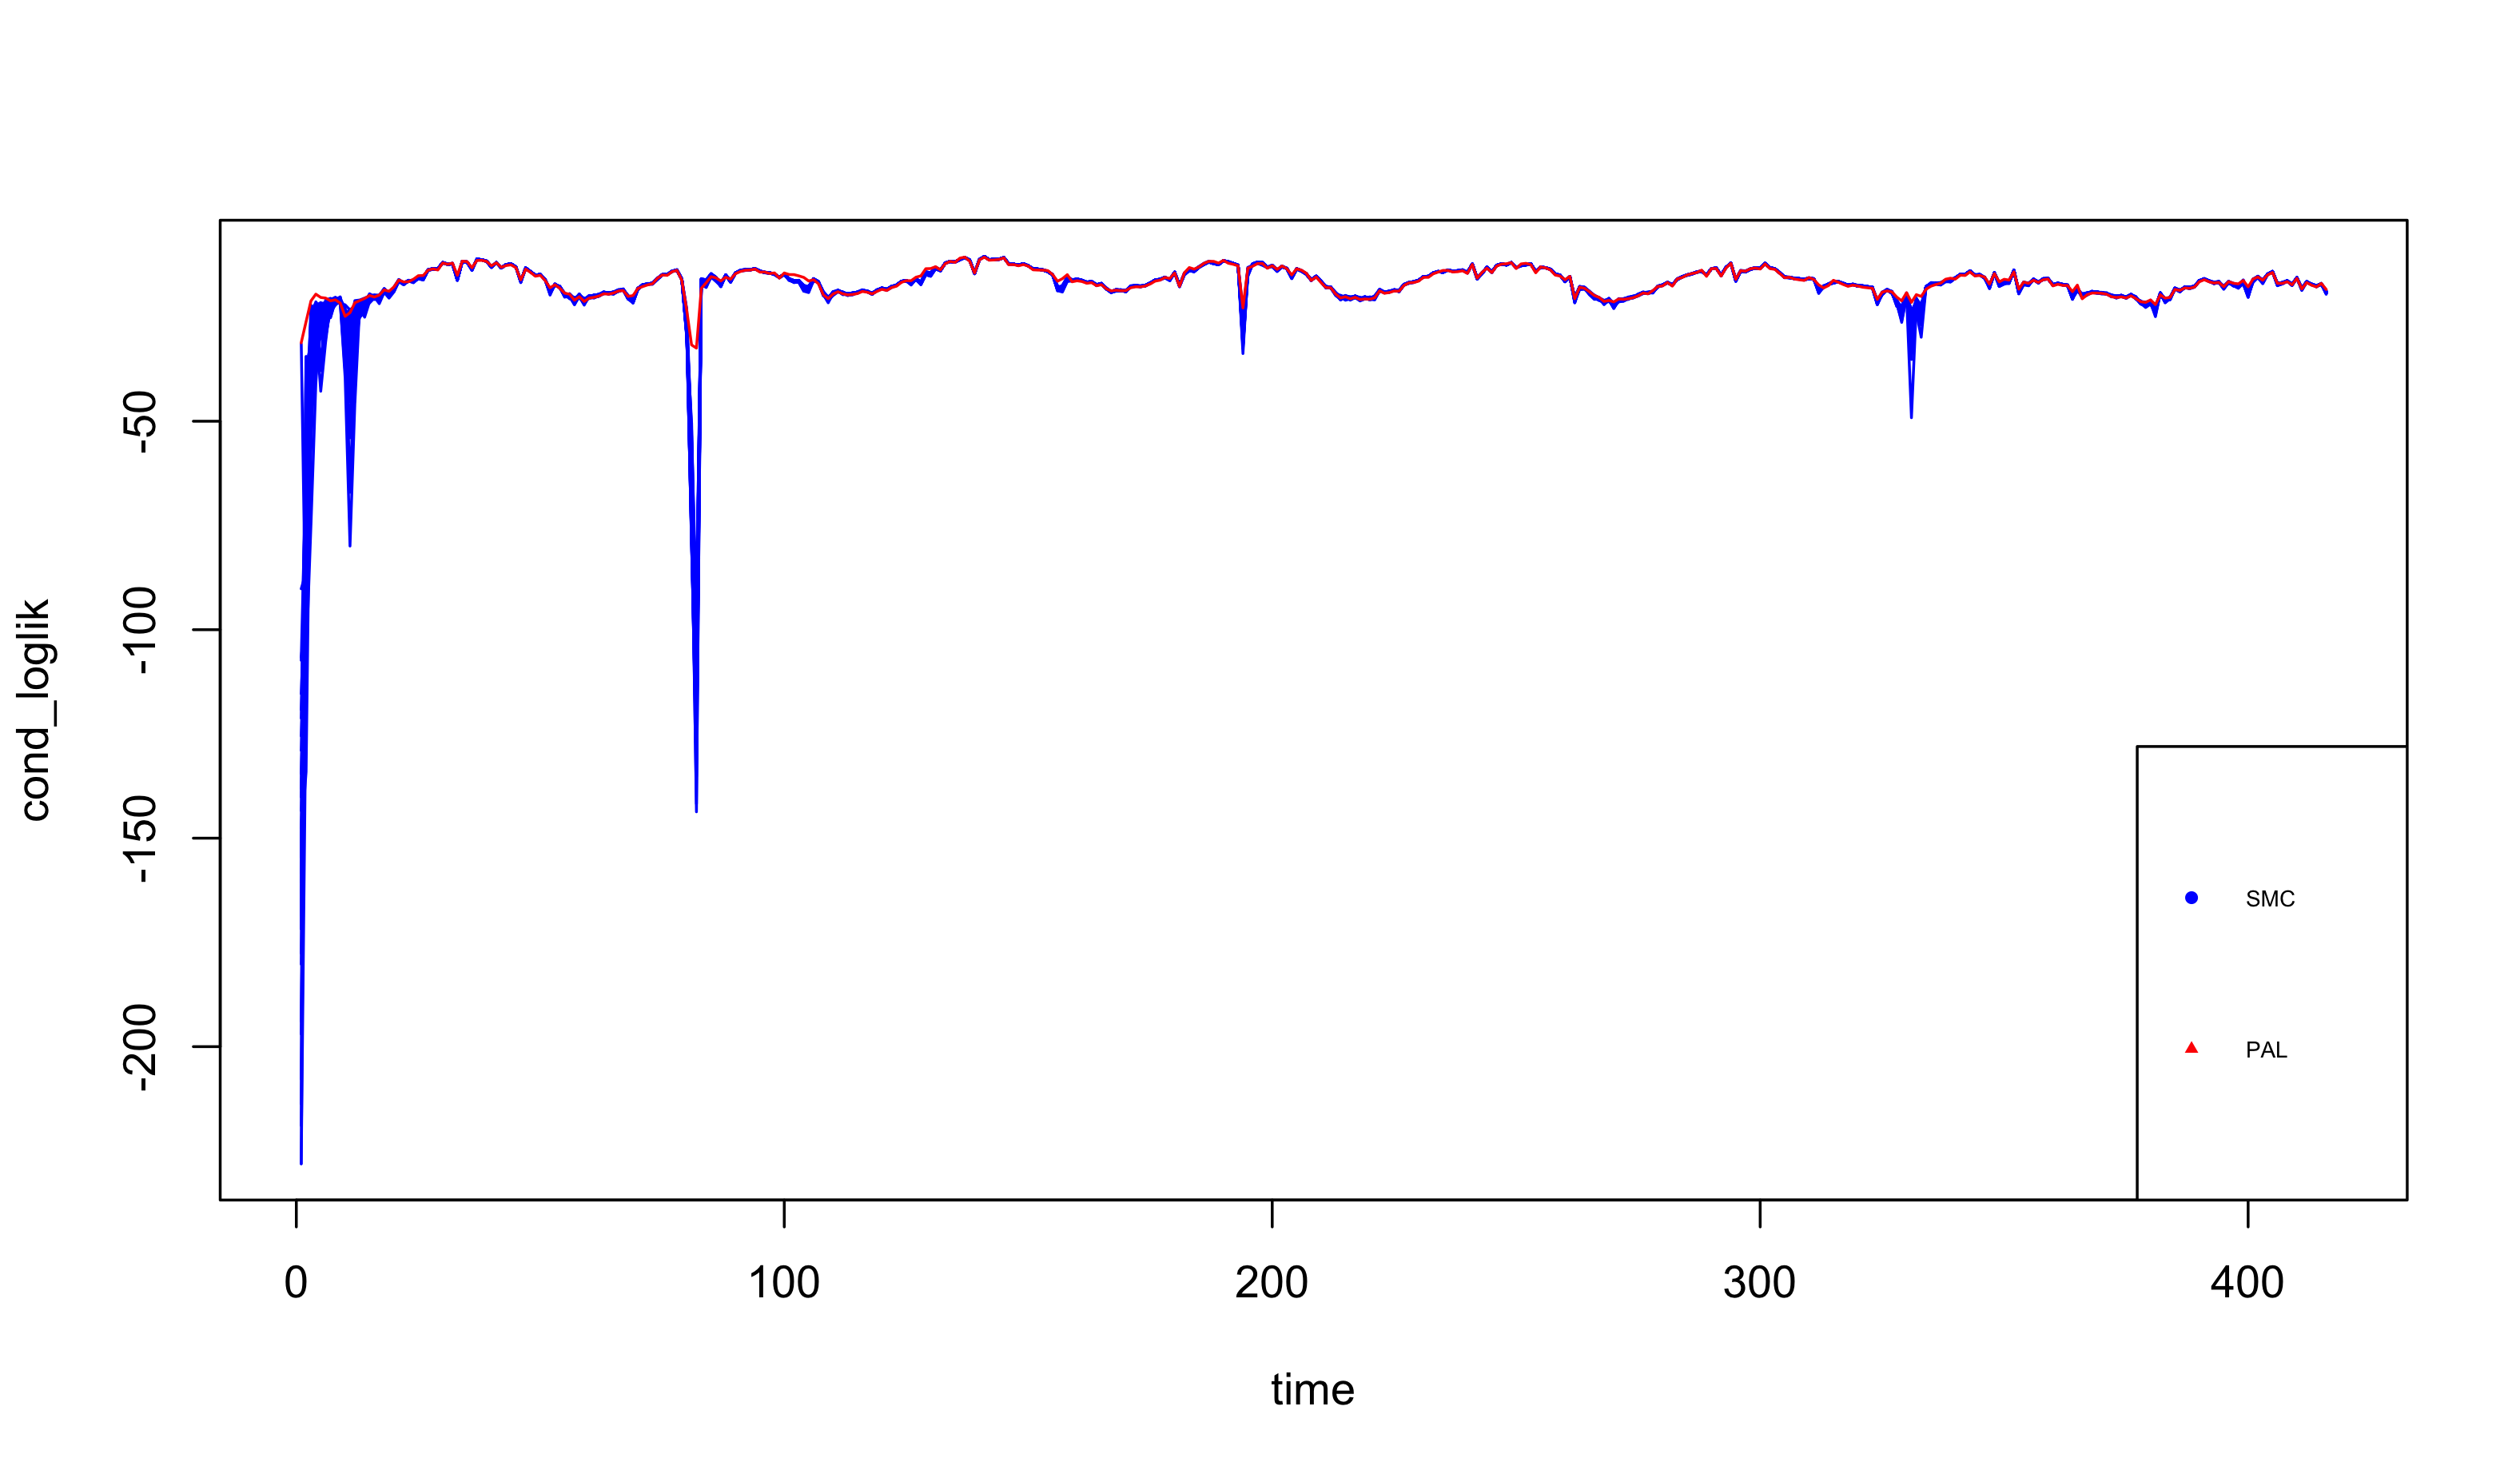
\includegraphics[width=0.9\textwidth]{cond_SMC_PAL_realdat.png}
\caption{\label{fig:cond_SMC_PAL_realdat}Conditional log-likelihoods computed using two methods for the real rotavirus dataset, with the SMC method replicated 36 times due to its high variances. The blue line represents overlapping results from 36 SMC computations, while the red line is derived from PAL. The main sources of likelihood shortfall of SMC are at time points $t=1, 2, 3, 11, 81, 194$, and $325-333$.}
\end{figure}

\vspace{-8mm}
\subsection{PAL versus SMC: When the Model is Correctly Specified}\label{section3}

Here, we utilize 100 simulated datasets from the OvOv model with parameters set at the MLE, thereby eliminating model misspecification. We then examine the likelihood values computed by PAL and SMC.


\begin{table}[htbp] % The placement specifier can be [h!tbp]
\centering % Centers the table
\caption{Average log-likelihood at the MLE at the 100 simulated datasets from OvOv computed by two filtering methods, employed 36 replicates and 50,000 particles} % This is effectively the table title
\label{tab:ovovtrue} % For referencing this table elsewhere in your text
\begin{tabular}{|c c c|} 
 \hline
  & PAL & SMC  \\ 
 \hline
 OvOv & -6231.97 & -6224.245 \\ 
 \hline
\end{tabular}
\end{table}
\begin{figure}[H]
\centering
\vspace{-7mm}
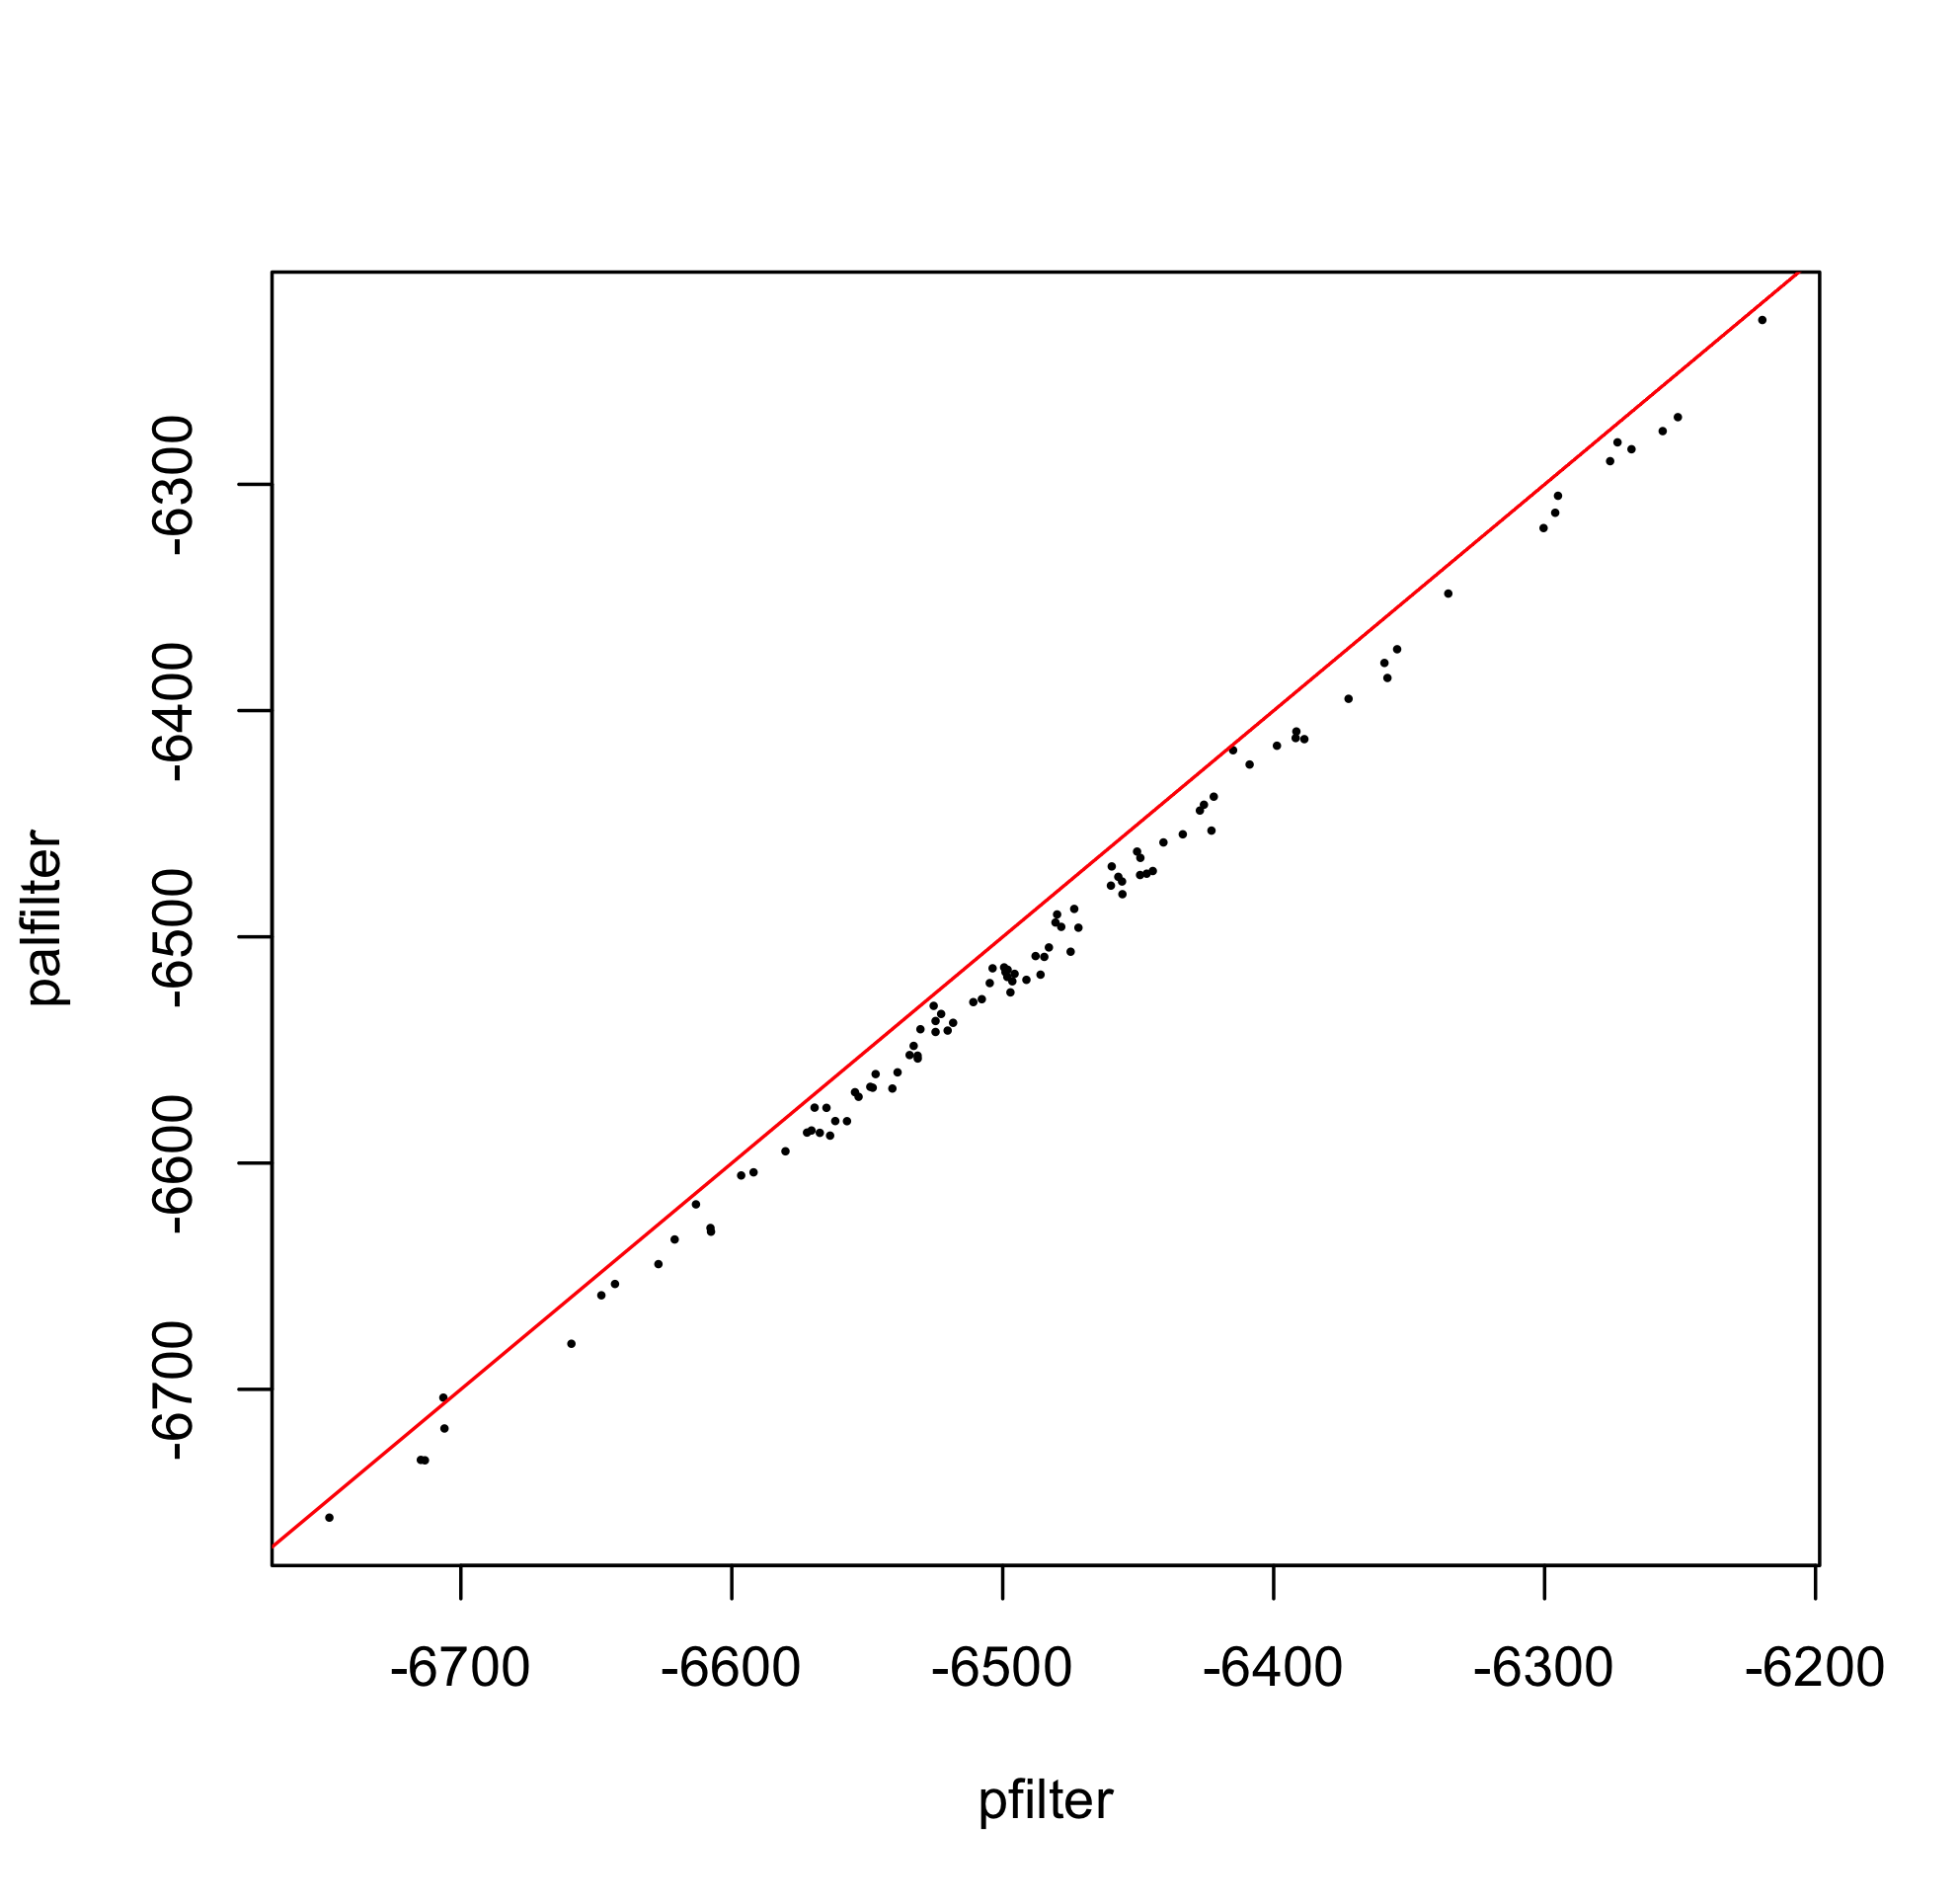
\includegraphics[width=0.55\textwidth]{PAL_vs_SMC_ovov_100.png}
\caption{\label{fig:PAL_vs_SMC_ovov_100}Log-likelihoods computed using two filtering methods for 100 randomly simulated datasets at the MLE of the OvOv model. The red line is the line $Lik(pfilter)=Lik(palfilter)$. We can see on the simulated data, SMC gives consistently higher likelihood estimates than PAL.}
\end{figure}



When the model is correctly specified, however, the log-likelihood values computed by PAL, as shown in Table \ref{tab:ovovtrue} and Figure \ref{fig:PAL_vs_SMC_ovov_100}, consistently exhibit a shortfall. This shortfall highlights the approximative nature of the PAL method compared to the more accurate SMC filter. It is posited that the model yielding the highest likelihood is, in theory, the true model, a concept we will explore in further detail in the discussion section \ref{dis}.

\subsection{Iterated Filtering Maximization of the Likelihood}

Besides proposing a novel filtering algorithm, by applying PAL to the model for rotavirus, \cite{wwr} claimed they have also identified a superior model, as a much lower AIC represented in Table \ref{tab:model_performance} indicates and the failure from getting a lower likelihood in Section \ref{misspecified}. However, as demonstrated in \ref{section3}, we recognize that SMC, functioning as an ideal filter, ought to yield a higher likelihood estimation when the model is correct. Notably, Section \ref{misspecified} reveals that when the model confronts actual rotavirus data, it encounters misspecification issues, particularly at times $t=1, \,\,2, \,\,3, \,\,11, \,\,81, \,\,194, \,\,325-333$, leading to shortfalls in likelihood. Appendix \ref{appendB} discusses this phenomenon, attributing it to certain data points that the model fails to adequately represent. This issue is especially pronounced at the initial time points. Particularly, in the initial time points $t=1,2,3$, the likelihood deviates from PAL estimates for about more than 100 log-likelihood units, suggesting an improper choice of initial distribution that might favor the PAL estimate. Consequently, we have opted to estimate the initial distribution \(\lambda_0 = (S_{10}, I_{10}, R_{10}, S_{20}, I_{20}, R_{20}, S_{30}, I_{30}, R_{30})\), where $S_{10}, I_{10}, R_{10}, S_{20}, I_{20}, R_{20}, S_{30}, I_{30}$, and $R_{30}$ represent the number of individuals in each compartment at time $t=0$. The results of this new estimation can be found in Table \ref{tab:mlebywwr}. Importantly, the maximization of the likelihood conducted via the Iterated Filtering (mif2) algorithm \citep{pomppackagepaper} procures a higher likelihood at the estimated MLE than that estimated by PAL, and a different yet comparable set of estimates is obtained. In terms of parameters pertinent to epidemiological interests, i.e. the first 7 rows in Table \ref{tab:mlebywwr}, we observe a lower force of infection parameter for the first age group, $\beta_1$, alongside a higher force of infection for the third age group, $\beta_3$. Additionally, we detect variations in the phase parameter $\phi$, which directly affects the seasonal time points, as well as in the stochastic parameter $\sigma_{\xi}$ and the initial compartmental distributions. The modifications to the initial distributions aim to rectify inadequate initialization, while the other adjustments address model misspecifications identified in Section \ref{misspecified}. Changes in the remaining parameter set are negligible. These findings indicate that when model misspecification is reduced to a minimal level, both PAL and SMC approaches tend to provide similar likelihood estimates, and the Iterated Filtering algorithm is capable of generating a superior maximum likelihood estimation than PAL equipped with the gradient ascent algorithm. Moreover, the results produced by SMC are more reliable due to the exact nature of the filter, despite PAL's computational efficiency.


\section{Discussion and Conclusion}\label{dis}

This paper examines two filtering approaches, with PAL specifically designed for certain types of compartmental POMP models. However, both methods have their limitations. Although this was not observed in our study, SMC is sensitive to model misspecification, which can lead to filtering failures. Conversely, PAL may experience a shortfall in likelihood estimation when the model is correctly specified.

PAL is an approximate filtering method used in scenarios where SMC is computationally prohibitive. It approximates the posterior distribution by a Poisson approximation. Due to its approximative nature, it does not perfectly capture the true posterior distribution. 
SMC, however, often referred to as the "perfect filter," uses a large set of particles and sophisticated resampling techniques to theoretically accurately approximate the posterior distribution. It is computationally more intensive than PAL but tends to provide a satisfying approximation, especially in complex models that are not compatible with PAL in general. When PAL and SMC are applied to a well-specified model meaning the model with the latent process model being correctly represented, SMC outperforms PAL because it better captures the nuances of the posterior distribution. This is why SMC might show a "likelihood shortfall" compared to PAL when the model is correctly specified. This is due to the approximation error of PAL can't be improved arbitrarily in general \citep{annurev:/content/journals/10.1146/annurev-control-042920-015119}, and likelihood being a proper scoring rule.

The concept of likelihood as a proper scoring rule \citep{gneiting1,gneiting2} in statistical models implies that using likelihood-based methods will naturally align with the true model of the data, assuming the model structure correctly represents the underlying process. When the likelihood function is used as a scoring rule, it is considered proper because maximizing the likelihood leads to parameter estimates that converge to their true values under large sample conditions, provided the model is specified correctly. A scoring rule is "strictly proper" if a forecaster maximizes the expected score by issuing a probabilistic forecast that exactly matches the true distribution of the outcomes. In other words, for a scoring rule to be strictly proper, the best strategy for the forecaster is to report the true probability distribution of the events they are forecasting. This promotes honest and accurate forecasting. This provides a theoretical explanation of why SMC outperforms PAL when the model is correct.

The "likelihood shortfall" in PAL when compared to SMC, particularly when the model is correct, highlights the trade-off between computational efficiency and accuracy in statistical approximations. While PAL may be faster and more computationally feasible in many scenarios, it sacrifices some accuracy, which becomes apparent when compared to the more exact SMC method, especially under the scrutiny of proper scoring rules as discussed in the context.

\section{Acknowledgement}

The code and results can be found on: \url{https://github.com/yhaoum/PAL-check.git}.

I would like to express my sincere gratitude to Prof. Ionides for selecting this interesting topic for me and providing consistent and immediate guidance throughout the entire process. I also want to extend my thanks to Aaron for dedicating his time to help review my code and results.

\newpage
\appendix
\section{Consistency of Models Built in \textbf{pomp} and \cite{wwr}}\label{appendA}

\begin{figure}[H]
\centering
\includegraphics[width=0.7\textwidth]{compare_density_plot_EqEq_old.png}
\caption{\label{fig:rotavirus} Density plot and t-test of mean, median, and variance of all three age-specific time series of 1000 Simulations from EqEq model built in WWR code and \textbf{pomp}}
\end{figure}

\begin{figure}[H]
\centering
\includegraphics[width=0.7\textwidth]{compare_density_plot_EqOv.png}
\caption{\label{fig:rotavirus} Density plot and t-test of mean, median, and variance of all three age-specific time series of 1000 Simulations from EqOv model built in WWR code and \textbf{pomp}}
\end{figure}

\begin{figure}[H]
\centering
\includegraphics[width=0.7\textwidth]{compare_density_plot_OvOv.png}
\caption{\label{fig:rotavirus} Density plot and t-test of mean, median, and variance of all three age-specific time series of 1000 Simulations from OvOv model built in WWR code and \textbf{pomp}}
\end{figure}


\section{Model Misspecification}\label{appendB}

\begin{figure}[H]
\centering
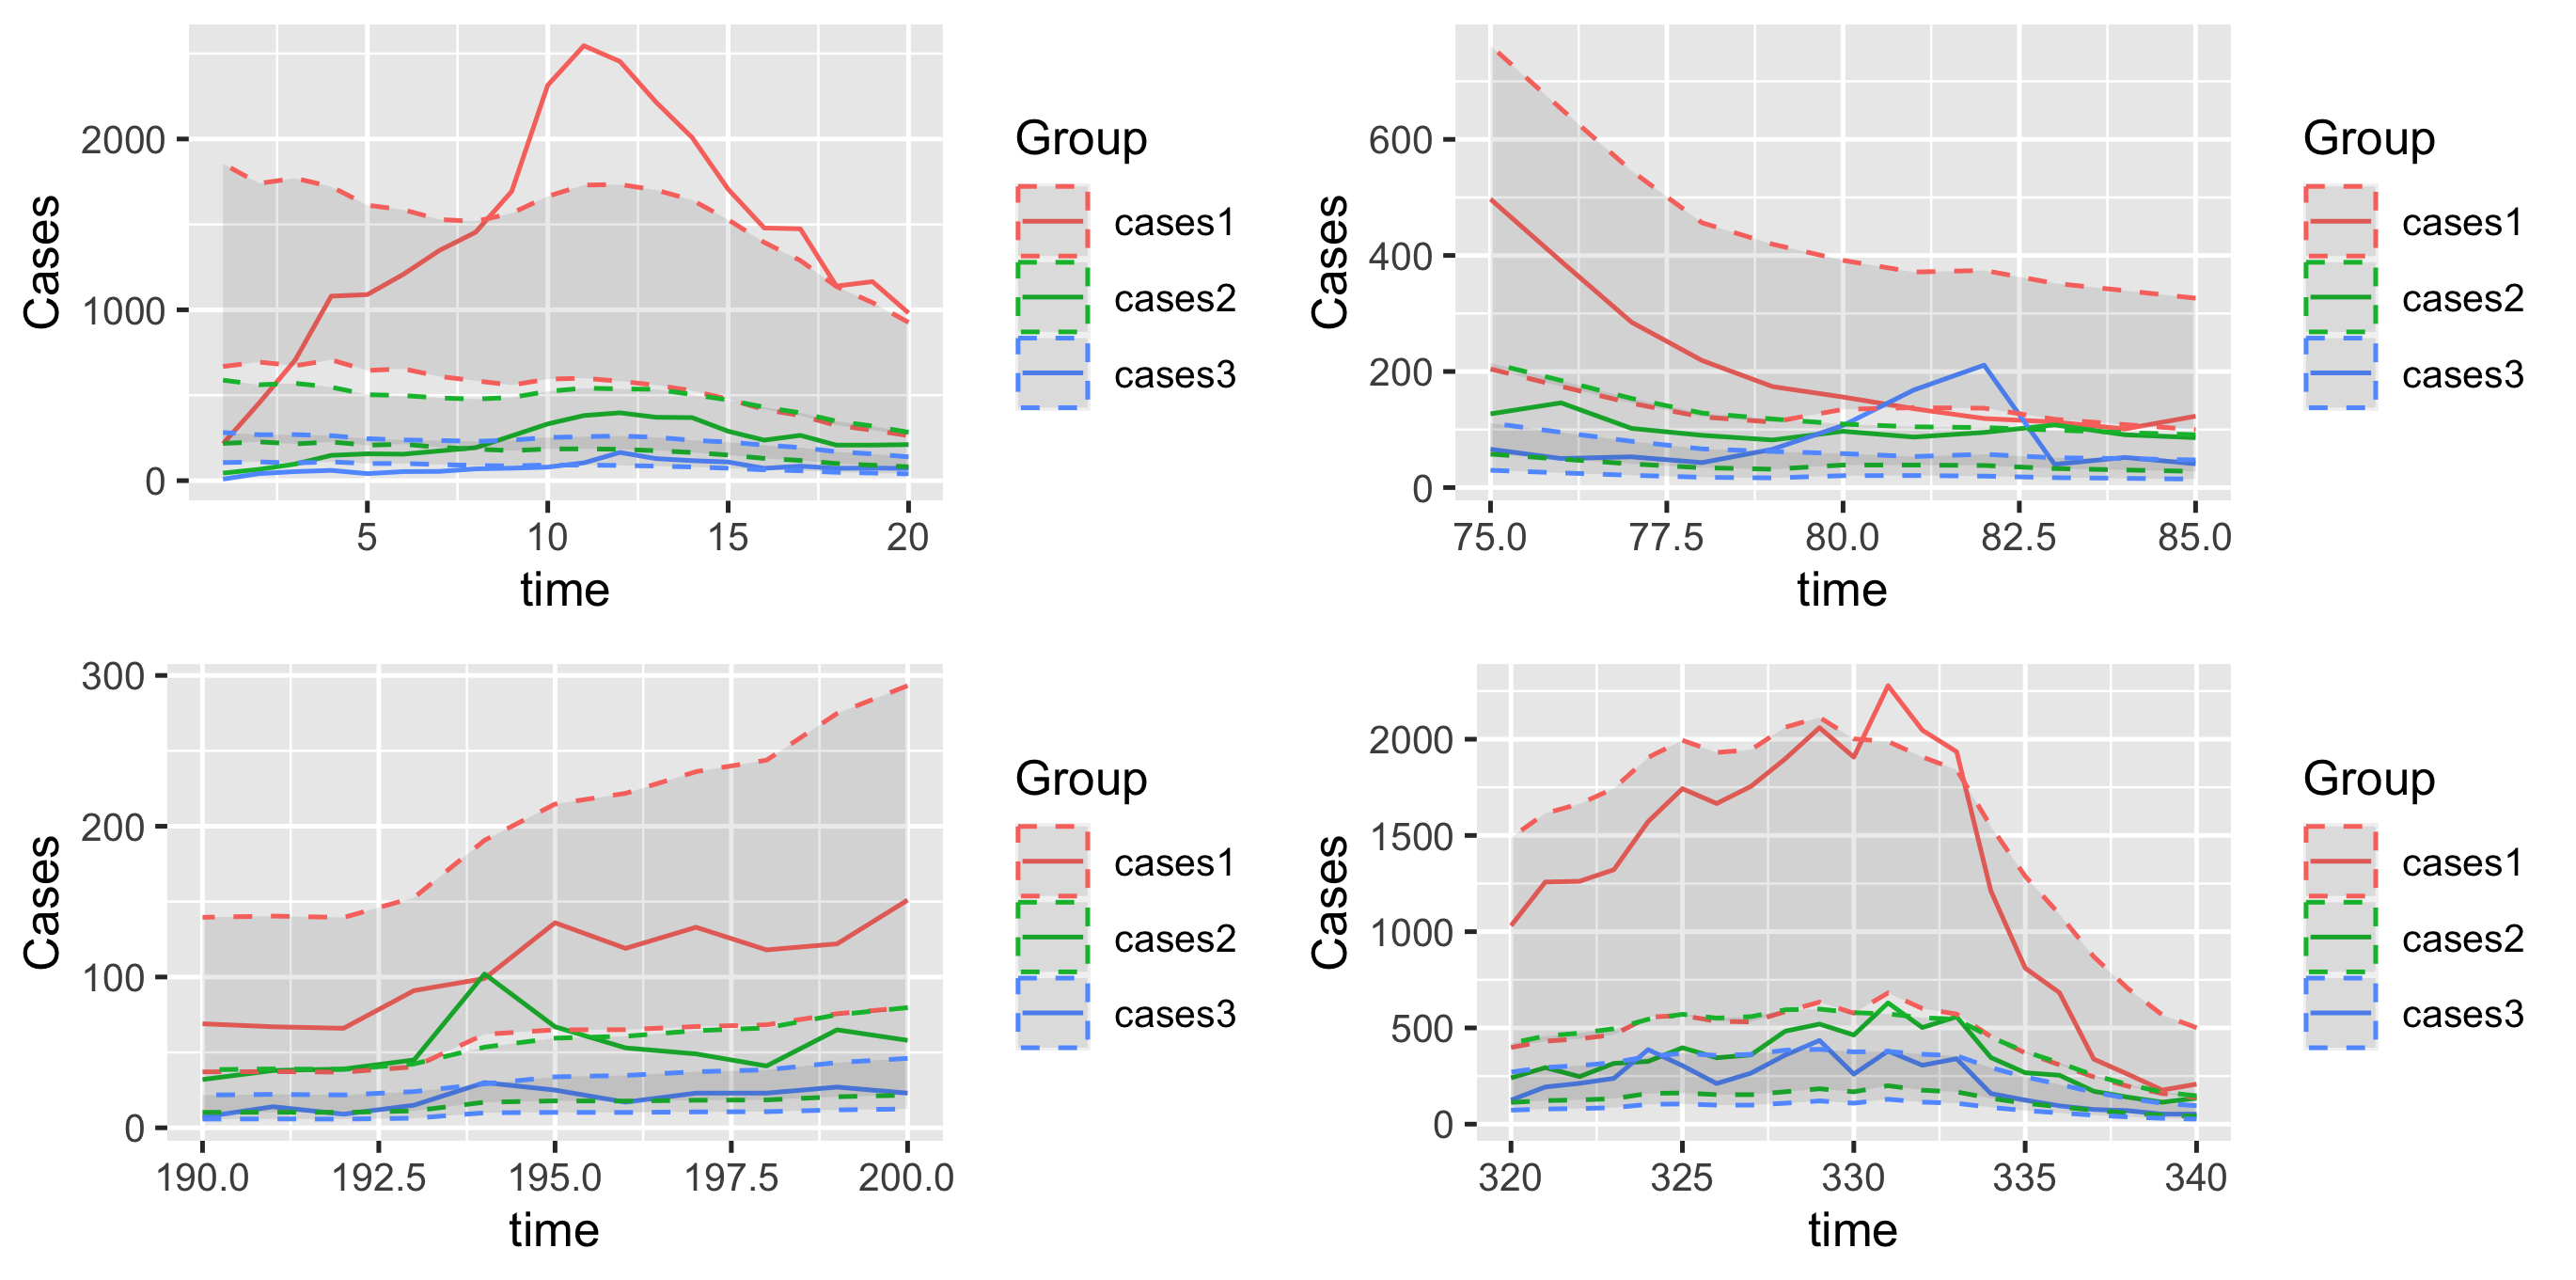
\includegraphics[width=\textwidth]{plot_zoom_png.png}
\caption{\label{fig:zoomedin_outlier_plot} Zoomed-in time-Cases plot at time $t=0-20, 75-85, 190-200$ and $320-340$. In the visualization, solid lines represent the true reported cases from the original rotavirus dataset, while the shaded strips with dashed boundaries-colored according to different groups—indicate enlarged "confidence intervals" for these cases. Specifically, the upper boundary of each strip corresponds to the upper 97.5\% percentile of 36 replicates of the filtered accumulated number of cases, $H_{kt}$, for $k=1,2,3$, and $t=1,2,...,416$, as introduced in Section \ref{observationmodel}. This boundary is further adjusted by the upper 97.5\% percentile of the reporting rate $q_t$, estimated by \cite{wwr} in Table \ref{tab:mlebywwr}. The reporting rate $q_t$ is assumed to follow a truncated normal distribution with a mean of 0.07 and a standard deviation of $\sigma_q = 0.021$, resulting in a lower 2.5\% percentile of 0.029 and an upper 97.5\% percentile of 0.111. The methodology for establishing the lower boundary of the strip mirrors that of the upper boundary. Although this approach is not entirely rigorous, each strip is intended to encompass our extended confidence interval for the true reported cases. Consequently, data points that fall outside these strips give us a intuition of where the model misspecifications may occur.}
\end{figure}

As illustrated in Figure \ref{fig:cond_SMC_PAL_realdat}, shortfalls are observed at times $t=1,\,\,2,\,\,3,\,\,11,\,\,81,\,\,194,$ and $325-333$. These discrepancies are primarily attributable to outliers that the model fails to accommodate. In the displayed results, it is immediately apparent that at the initial times $t=1, \,\,2, \,\,3$ all the true reported cases deviated from the expected range, falling outside the designated strip. Specifically, at time $t=11$, the model is misspecified for case 1, depicted by the solid red line. Similarly, at times $t=81,\,\, 82$, the model is misspecified for case 3, as indicated by the solid blue line that extended beyond the strip's boundaries. At $t=194$, the solid green line denotes case 2 as where the model is misspecified. During the period from $t=325-333$, all three observed cases are where the model misspecifications happen. These deviations provide a clear illustration of the likelihood shortfall of the sequential Monte Carlo (SMC) method when the model does not align with the data, suggesting a model misspecification. 

\newpage
\bibliography{sample.bib}

\end{document}
